\documentclass[12pt,a4paper]{extreport}
\usepackage[l2tabu,orthodox]{nag}
\usepackage{subcaption}

% Пожалуйста, не меняйте указанные ниже установки полей в документе
\usepackage[left=10mm,right=10mm, top=15mm,bottom=15mm,bindingoffset=0cm]{geometry}

\usepackage{indentfirst}
\usepackage{float}

%\usepackage{ccaption}
%\captiondelim{. }

\usepackage{amssymb,amsmath,amsthm}

\usepackage{fontspec}
%\usepackage{unicode-math}

\setmainfont[Ligatures=TeX]{STIX}
\newfontfamily{\cyrillicfont}[Ligatures=TeX]{STIX}
\setmonofont{Fira Mono}
\newfontfamily{\cyrillicfonttt}{Fira Mono}

\usepackage{polyglossia}
\setdefaultlanguage{russian}
\setotherlanguage{english}


\usepackage{graphicx}
\graphicspath{{img/}}
\DeclareGraphicsExtensions{.pdf,.png,.jpg}


\usepackage{color}
\definecolor{darkblue}{rgb}{0,0,.75}
\definecolor{darkred}{rgb}{.7,0,0}
\definecolor{darkgreen}{rgb}{0,.7,0}

\usepackage[normalem]{ulem}
\usepackage[textwidth=4cm,textsize=tiny]{todonotes}
\newcommand{\fix}[2]{{\textcolor{red}{\uwave{#1}}\todo[fancyline]{#2}}}
\newcommand{\hl}[1]{{\textcolor{red}{#1}}}
\newcommand{\cmd}[1]{{\ttfamily{\textbackslash #1}}}
\usepackage[pverb-linebreak=no]{examplep}
\newcommand{\vrb}[1]{\PVerb{#1}}
\newcommand{\vrbb}[1]{\texttt{\textbackslash}\PVerb{#1}}
\newcommand{\rulez}{{\href{https://goo.gl/FhyJJm}{Правила}}}

\usepackage[
    draft = false,
    unicode = true,
    colorlinks = true,
    allcolors = blue,
    hyperfootnotes = true
]{hyperref}


\theoremstyle{plain}
\newtheorem{theorem}{Теорема}
\newtheorem{lemma}{Лемма}
\newtheorem{proposition}{Утверждение}
\newtheorem{corollary}{Следствие}
\theoremstyle{definition}
\newtheorem{definition}{Определение}
\newtheorem{notation}{Обозначение}
\newtheorem{example}{Пример}
    
\newenvironment{task}[1]
    {\par\noindent\textbf{Задача \href{http://progensys.dainiak.com/problem-#1}{#1}. }}
    {\smallskip}
\newenvironment{solution}
    {\par\noindent\textbf{Решение. }}
    {\bigskip}

\title{Решения задач по курсу «Дискретные структуры»}
\author{Константин Леладзе}

\begin{document}
\maketitle

% Таким образом нужно добавлять решения задач:

\begin{task}{99}
Решите сравнение $52x\equiv 48\pmod{404}$. Решение необходимо записать по модулю 404. Для решения задачи нахождения обратного по умножению элемента продемонстрируйте применение алгоритма Евклида. Перебор/угадывание не допускаются.
\end{task}

\begin{solution}
Для начала, запишем общий вид уравнения: $ax\equiv b\pmod{m}$. В нашем случае: $a = 52 ,\, b = 48 ,\, m = 404$. Найдем $d = \operatorname{gcd}(a, m)$:
\begin{align*}
    404/52 = 7 \text{, остаток } 40;\\
    52/40 = 1 \text{, остаток } 12;\\
    40/12 = 3 \text{, остаток } 4;\\
    12/4 = 3 \text{, остаток } 0;\\
    d = \operatorname{gcd}(52, 404) = 4.\newline
\end{align*}
\par
Исходное уравнение упрощается до $ax/d\equiv b/d\pmod{m/d}$, если $d\mathop{|}b$.
В нашем случае $48/4 = 12$. Получаем: $13x\equiv 12 \pmod{101}$.
\par
\begin{align*}
    101 = 7\cdot13 + 10;\\
    13 = 1\cdot10 + 3;\\
    10 = 3\cdot3 + 1;\\
    3 = 3\cdot1 + 0.
\end{align*}\par
Используя обратный проход (аналог РАЕ):
\begin{gather*}
1 = 10 - 3\cdot\uline{3} = \\
1\cdot\uline{10} - 3\cdot(13 - 1\cdot\uline{10}) = -3\cdot13 + 4\cdot\uline{10} = \\
-3\cdot\uline{13} + 4\cdot(101 - 7\cdot\uline{13}) = 4\cdot101 + (-31\cdot\uline{13}) \equiv \\
70\cdot\uline{13} \pmod{101}.
\end{gather*}\par
Значит, обратный по модулю 101 к $13$ элемент --- $70$.\par
Имеем $x_0 = 12\cdot13^{-1}=12\cdot70\equiv 32 \pmod{101}$.\par
\par
С учетом того, что исходное уравнение нужно решить по модулю $404$:
\begin{gather*}
x \equiv x_0 + 101 \cdot k \pmod{404} ,\, k \in \{0, 1, \dots, d - 1\};\\
x \equiv {32, 133, 234, 335} \pmod{404}.
\end{gather*}
\end{solution}
\begin{task}{102}
Решите сравнение $71x\equiv 12\pmod{269}$. Для решения задачи нахождения обратного по умножению элемента продемонстрируйте применение алгоритма Евклида. Перебор/угадывание не допускаются.
\end{task}

\begin{solution}
Для начала, запишем общий вид уравнения: $ax\equiv b\pmod{m}$. В нашем случае: $a = 71 ,\, b = 12 ,\, m = 269$. Найдем $d = \operatorname{gcd}(a, m)$:
\begin{align*}
    269 = 3\cdot71 + 56;\\
    71 = 1\cdot56 + 15;\\
    56 = 3\cdot15 + 11;\\
    15 = 1\cdot11 + 4;\\
    11 = 2\cdot4 + 3;\\
    4 = 1\cdot3 + 1;\\
    3 = 3\cdot1 + 0.\\
    d = \operatorname{gcd}(71, 269) = 1.
\end{align*}
\par
Используя обратный проход (аналог РАЕ):
\begin{gather*}
1 = 4 - 1\cdot\uline{3} = \\
1\cdot\uline{4} - 1\cdot(11 - 2\cdot\uline{4}) = -11 + 3\cdot\uline{4} = \\
-1\cdot\uline{11} + 3\cdot(15 - 1\cdot\uline{11}) = 3\cdot15 - 4\cdot\uline{11} = \\
3\cdot\uline{15} - 4\cdot(56 - 3\cdot\uline{15}) = -4\cdot56 + 15\cdot\uline{15} = \\
-4\cdot\uline{56} + 15\cdot(71 - 1\cdot\uline{56}) = 15\cdot71 - 19\cdot\uline{56} = \\
15\cdot\uline{71} - 19\cdot(269 - 3\cdot\uline{71}) = -19\cdot269 + 72\cdot\uline{71} \equiv \\
72\cdot\uline{71} \pmod{269}.
\end{gather*}\par
Значит, обратный по модулю $269$ к $71$ элемент --- $72$.\par
Имеем $x_0 = 12\cdot71^{-1}=12\cdot72\equiv 57 \pmod{269}$.\par
Ответ: $x = 57 + 269k$, где $k \in \mathbb{Z}$.
\end{solution}
\begin{task}{104}
Существует ли $k$, такое, что $13^k$ оканчивается на $\dots0000169$?
\end{task}

\begin{solution}
Да: $k = 4000002$. Это можно понять, решив сравнение $13^{k-2} \equiv 1 \pmod{10^7}$. Оно эквивалентно исходному, так как $\operatorname{gcd}(13, 10) = 1$.\par
По теореме Эйлера:
\begin{equation*}
    13^{\varphi(m)}\equiv 1 \pmod{10^7}.
\end{equation*}
Вычислим $\varphi(m)$:
\begin{gather*}
    \varphi(m) = \varphi(2^7\cdot5^7) = m\cdot\left(1-\frac{1}{2} \right) \cdot\left(1-\frac{1}{5} \right)=4\cdot10^6.
\end{gather*}
Таким образом:
\begin{equation*}
    k - 2 = 4\cdot10^6.
\end{equation*}
Отсюда, $k = 4000002$ нам подходит.
\end{solution}
\begin{task}{138}
Найдите хотя бы один первообразный корень по модулю $11^{1000}$.
\end{task}

\begin{solution}
Для начала, запишем определение первообразного корня $g$ по модулю $m$:
\begin{equation*}
    \forall a \in \mathbb{Z} \ \text{т.ч.} \operatorname{gcd}(a, m) = 1 \ \exists k \in \mathbb{Z} : g^{k} \equiv a \pmod{m}.
\end{equation*}
Вспомним, что можно воспользоваться следующим утверждением:

\begin{theorem} \label{(g+mx)^(m-1)_prim_roots}
Если $g$ --- первообразный корень по простому модулю $m$, то $\exists \ x \ \forall \alpha \geq 1 : g+m\cdot x$ --- первообразный корень по модулю $m^\alpha$. Подходят именно $x$, такие, что: ${\left( g+m\cdot x \right)}^{m - 1} = 1 + m \cdot y$, где $\operatorname{gcd}(y, m) = 1$.
\end{theorem}

Чтобы воспользоваться этой теоремой \ref{(g+mx)^(m-1)_prim_roots} --- найдем сначала первообразный корень по модулю 11. Докажем, что $2$ --- первообразный корень по модулю 11, перебрав все $a \in \{1,2,3,4,5,6,7,8,9,10\}$:
\begin{enumerate}
    \item $a = 1$: \\
    возьмем $k = 10$:  $2^{10} = 1024 \equiv 1 \pmod{11};$
    \item $a = 2$: \\
    возьмем $k = 1$:  $2^1 = 2 \equiv 2 \pmod{11};$
    \item $a = 3$: \\
    возьмем $k = 8$:  $2^8 = 256 \equiv 3 \pmod{11};$
    \item $a = 4$: \\
    возьмем $k = 2$:  $2^2 = 4 \equiv 4 \pmod{11};$
    \item $a = 5$: \\
    возьмем $k = 4$:  $2^4 = 16 \equiv 5 \pmod{11};$
    \item $a = 6$: \\
    возьмем $k = 9$:  $2^9 = 512 \equiv 6 \pmod{11};$
    \item $a = 7$: \\
    возьмем $k = 7$:  $2^7 = 128 \equiv 7 \pmod{11};$
    \item $a = 8$: \\
    возьмем $k = 3$:  $2^3 = 8 \equiv 8 \pmod{11};$
    \item $a = 9$: \\
    возьмем $k = 6$:  $2^6 = 64 \equiv 9 \pmod{11};$
    \item $a = 10$: \\
    возьмем $k = 5$:  $2^5 = 32 \equiv 10 \pmod{11}.$
\end{enumerate}

Теперь можно воспользоваться теоремой~\ref{(g+mx)^(m-1)_prim_roots}:
\begin{equation*}
    {\left( 2 + 11\cdot x \right)}^{10} = 1 + 11\cdot y, \text{ при} \operatorname{gcd}(y, 11) = 1.
\end{equation*} \par
Подставив $x = 0$, получим:
\begin{equation*}
    {\left( 2 + 11\cdot 0 \right)}^{10} = 1024 = 1 + 11\cdot 93.
\end{equation*} \par
Значит, $y = 93$. Осталось проверить, что $\operatorname{gcd}(93, 11) = 1$:
\begin{align*}
    93 = 8\cdot11 + 5;\\
    11 = 2\cdot5 + 1;\\
    5 = 5\cdot1 + 0;\\
    \operatorname{gcd}(93, 11) = 1.
\end{align*}
Получается, действительно, $g = 2$ --- первообразный корень по модулю $11^{1000}$.
\end{solution}

\begin{task}{155}
Пусть $f,\,g,\,h$ -- неубывающие функции из $\mathbb{R}^+$ в $\mathbb{R}^+$. Пусть $n \to \infty$. Верно ли, что если $f(n)=O(g(n))$ и $g(n)=o(h(n))$, то обязательно $f(n)=o(h(n))$? Если верно, то обоснуйте, опираясь исключительно на определения. Если не верно в общем случае, то приведите соответствующий контрпример.
\end{task}

\begin{solution}
Вспомним определения $o$-малого и $O$-большого: \par
Пусть $f(x)$ и $g(x)$ — две функции, определенные в $U_\varepsilon(x_0)$ и $\lim_{x\to x_0} g(x) \neq 0$. Тогда говорят, что: \newline
$f = O(g)$, при $x \to x_0$, если $\exists C > 0 : \forall x \in U_\varepsilon(x_0) \Rightarrow |f(x)| \leq C|g(x)|$.\newline
$f = o(g)$, при $x \to x_0$, если $\forall c > 0,\, \exists \delta > 0 : \forall x \in U_\delta(x_0) \Rightarrow |f(x)| < c|g(x)|$.
\newline \newline
Теперь, с учетом того, что $f,\,g,\,h$ -- неубывающие функции и $x_0 = + \infty$:\par
(1) $\exists C > 0$ и $\exists x_1 \neq + \infty : \forall x > x_1 \Rightarrow |f(x)| \leq C|g(x)|$.\par
(2) $\forall c > 0 \exists x_2 \neq + \infty : \forall x > x_2 \Rightarrow |g(x)| < c|h(x)|$.\newline
Возьмем в (2) $c = C$. Пусть также $x_3(c) = \max(x_1, x_2(c))$. Тогда выполнено: $\forall x > x_3: |f(x)| \leq C|g(x)| < C^2|h(x)|$. \newline
Значит $\forall c > 0 \exists x_3(c) \neq + \infty : \forall x > x_3 \Rightarrow |f(x)| < C'|h(x)|$ (тут $C' = C^2$).\newline
Отсюда $f(n)=o(h(n))$.
\end{solution}
\begin{task}{157}
Пусть в двудольном графе $G$ с долями $X$ и $Y$ существует совершенное паросочетание, и пусть $\operatorname{deg} v \geq t$ для каждой вершины $v \in X$. Докажите, что в $G$ найдутся не менее $t!$ различных совершенных паросочетаний.
\end{task}

\begin{solution}
В $G$ есть совершенное пароочетание по условию. Значит, доли $X$ и $Y$ имеют одинаковую мощность. Помимо этого, выполняются условия Холла: $\forall \ U \subset X : |N(U)| \geq |U|$. Будем использовать конструктивный метод доказательства, а именно --- индукцию. \\
База: $|X| = |Y| = 1$: $\forall \ u \in X: \operatorname{deg}(v) = 1, \exists \ !$ \text{паросочетание}. \\
Чтобы доказать переход, придется рассмотреть два случая:
\begin{enumerate}
    \item $\exists \text{ непустое } \ U_1 \subset X \text{ (включение строгое)} : |N(U_1)| = |U_1|$. Далее, докажем существование совершенного паросочетания не только в $G$, но и в $G'(V'_1, V'_2)$, где $V'_1 = X \setminus U_1$, $V'_2 = Y \setminus N(U_1)$. Обозначим это паросочетание за $P$. \par
    Рассмотрим множество $U_2 \subset (X \setminus U_1)$. Известно (по условию), что в графе $G$ существует совершенное паросочетание. Это дает нам $|U_2| \leq |N(U_2)|$ и $|N(U_1 \ \cup \ U_2)| \geq |U_1 \ \cup \ U_2| = |U_1| + |U_2|$. По определению множества $U_1$, имеем $|N(U_2) \setminus N(U_1)| \geq |U_2|$. Значит, $|N(U_2) \ \cap \ (Y \setminus N(U_1))| \geq |U_2|$. Получается, что и для графа $G'$ выполнены условия Холла. Значит, в нем действительно существует совершенное паросочетание $P$.\par
    Докажем, теперь, собственно, переход индукции. Итак, по предположению --- в графе $G''(U_1, N(U_1))$ существует не менее $t!$ различных совершенных паросочетаний (степени вершин $U_1$ в подграфе такие же, как во всем графе, условия Холла также выполнены). В исходном графе $G$ также будет не меньше чем $t!$ совершенных паросочетаний: добавим найденное нами совершенное паросочетание $P$ ко всем совершенным паросочетаниям в $G''$.
    
    \item $\forall \text{ непустого } \ U_1 \subset X \text{ (включение строгое) } : |N(U_1)| > |U_1|$.\par
    Рассмотрим произвольную вершину $u \in X$. По условию --- $\operatorname{deg}(u) = n \geq t$. Удалим из графа вершину $u$ и какую-нибудь вершину $v$, такую что: $v \in N(\{u\})$. Заметим, что условия Холла не нарушаются, ведь величина \\ $|N(U_1)|$ уменьшается максимум на один для любого непустого подмножества $U_1 \subset X \setminus \{u\}$. При этом $\forall \ w \in X \setminus \{u\} : \operatorname{deg}(w) \geq (t - 1)$. Значит, в графе $G'(X \setminus \{u\}, Y \setminus \{v\} $ существует не менее $(t - 1)!$ совершенных паросочетаний.\par
    Значит, в исходном графе ($G$) существует не менее $(t - 1)!$ совершенных паросочетаний. Причем, каждое из них содержит $\{u, v\}$, где $v \in N(\{u\})$. \\ Очевидно, $|{\{u, v\} : v \in N(\{u\})}| = n \geq t$. Получим, что в исходном графе $G$ будет уже как минимум $t!$ совершенных паросочетаний.
\end{enumerate}
Переход доказан, а вместе с ним и решена задача.

\end{solution}\par

\begin{task}{202}
В чемпионате хоккейной лиги расписание регулярного чемпионата составляется по следующему правилу: не обязательно каждый клуб играет со всеми другими, но среди любых трёх клубов хотя бы два из них должны сыграть матч между собой и никакая пара клубов не играет друг с другом больше одного раза. Всего в лиге играют $26$ клубов. Верно ли, что, как бы ни было составлено расписание, найдётся семь клубов, каждые два из которых играли матч друг с другом?
\end{task}

\begin{solution}
Рассмотрим неориентированный граф, с вершинами, в которых находятся клубы, и ребрами, которые существуют между двумя вершинами, если клубы, соответствующие этим вершинам, играли.\par
Среди любых трех клубов найдутся два, которые играли друг с другом, значит в графе не будет независимых множеств на трех и более вершинах.
\begin{enumerate}
\item Оценим $R(7, 3)$, используя свойства чисел Рамсея:
\[R(7, 3) \leq R(7, 2) + R(6, 3) = 7 + R(6, 3).\]

\item Оценим $R(6, 3)$, используя свойства чисел Рамсея:
\[R(6, 3) \leq R(6, 2) + R(5, 3) - 1 = 6 + R(5, 3) - 1 = 5 + R(5, 3).\]
Тут также предположили, что $R(5, 3)$ --- четное. Докажем это далее. 

\item Оценим $R(5, 3)$, используя свойства чисел Рамсея:
\begin{gather*}
R(5, 3) \leq R(5, 2) + R(4, 3) = 5 + R(4, 3);\\
R(5, 3) \leq 5 + R(4, 2) + R(3, 3) - 1 = 5 + 4 + 6 - 1 = 14;\\
R(5, 3) \leq 14.
\end{gather*}

\item Приведем пример, который покажет, что $14 \leq R(5, 3)$.
Для этого, построим два графа на $13$ вершинах: без независимых множеств размера $5$ и без клик размера $3$ соответственно.
\begin{figure}[H]
  \centering
  \begin{subfigure}[a]{0.24\linewidth}
    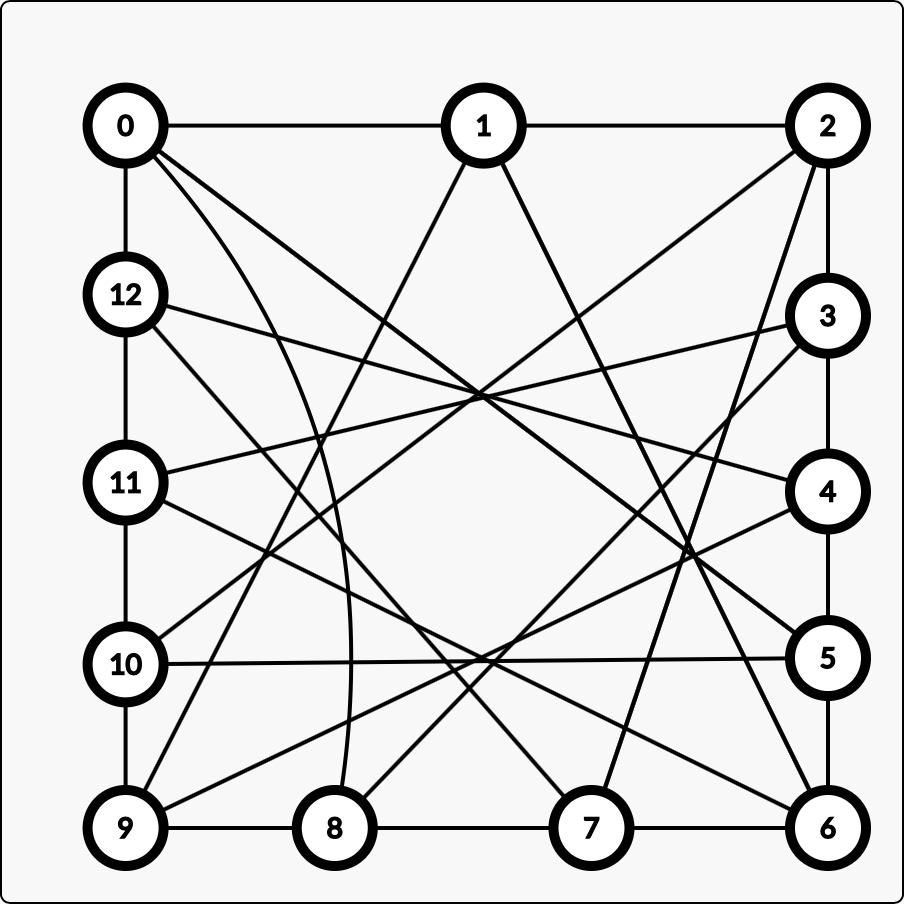
\includegraphics[width=\linewidth]{_img/202/01.png}
  \end{subfigure}
  \caption{граф без независимых множеств из пяти вершин.}
\end{figure}
\begin{figure}[H]
  \centering
  \begin{subfigure}[a]{0.24\linewidth}
    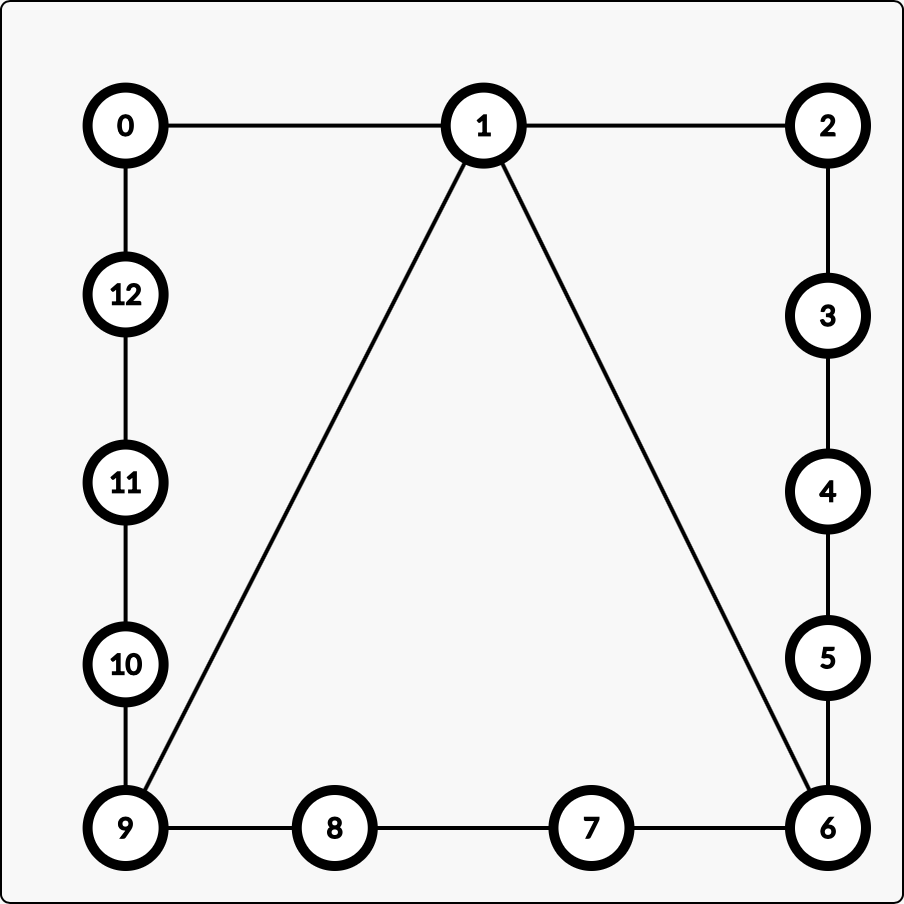
\includegraphics[width=\linewidth]{_img/202/02.png}
  \end{subfigure}
  \caption{граф без клик из трех вершин}
\end{figure}

\item
Получается, что
\begin{gather*}
    R(5, 3) = 14;\\
    R(6, 3) \leq 19;\\
    R(7, 3) \leq 26.
\end{gather*}
\end{enumerate}
Значит, в графе на $26$ вершинах найдется либо независимое множество размера $3$, либо клика размера $7$. По условию, независимых множеств размера $3$ в графе нет. Значит, среди каких-то семи команд каждые две играли между собой.
\end{solution}
\begin{task}{222}
Для многочлена $x^4 + x^3 + x^2 + 1$ над полем $\mathbb{Z}_3$ определите, является ли он неприводимым.
\end{task}

\begin{solution}
Многочлен четвертой степени неприводим, если он не имеет корней и не делится на многочлен второй степени.
\begin{enumerate}
\item Очевидно, корней у данного многочлена нет. Все возможные числа поля $0$, $-1$ и $1$ не являются корнями.

\item Предположим, что данный многочлен делится на какой-то многочлен второй степени: $x^4 + x^3 + x^2 + 1 = (ax^2 + bx + c)\cdot(dx^2 + ex + f)$. Выразим коэффициенты:
\begin{equation*}
    \begin{cases}
        ad = 1;\\
        ae + bd = 1;\\
        af + be + cd = 1;\\
        bf + ce = 0;\\
        cf = 1.
    \end{cases}
\end{equation*}
Докажем, что данная система не имеет решений для натуральных чисел $a, b, c, d, e, f$.\par
Из первого уравнения: $a = \frac{1}{d}$. Подставим в систему:
\begin{equation*}
    \begin{cases}
        \frac{e}{d} + bd = 1;\\
        \frac{f}{d} + be + cd = 1;\\
        bf + ce = 0;\\
        cf = 1.
    \end{cases}
\end{equation*}
Из четвертого уравнения: $c = \frac{1}{f}$. Из третьего: $b = -\frac{ce}{f} = -\frac{e}{f^2}$ Подставим в систему:
\begin{equation*}
    \begin{cases}
        \frac{e}{d} - \frac{e}{f^2} = 1;\\
        \frac{f}{d} - \frac{e}{f^2} + \frac{d}{f} = 1.
    \end{cases}
\end{equation*}
Из певрого уравнения: $e = \frac{f^2d}{f^2 - d}$. Подставим в систему:
\begin{equation*}
     \frac{f}{d} - \frac{f^4d^2}{(d^2-d)^2} + \frac{d}{f} = 1.
\end{equation*}
Упростим:
\begin{equation*}
     (f^2 - df +d^2)(f^2 - d)^2 = f^5d^3\\.
\end{equation*}
Это уравнение не имеет решений в натуральных числах.
\end{enumerate}
\par Значит исходный многочлен неприводим.
\end{solution}
\begin{task}{238}
На курсе $100$ студентов. Известно, что среди них можно выделить 
$149$ различных пар студентов, которые во время семестра давали друг другу списывать на контрольных. Деканат принял решение отчислить после сессии минимально возможное число студентов, но таким образом, чтобы среди оставшихся студентов не осталось ни одной пары списывающих друг у друга. Докажите, что к следующему семестру на курсе останется не менее $26$ студентов.
\end{task}

\begin{solution}
Возьмем граф $G$ на $100$ вершинах (соответствуют студентам). Ребро $e = \{u, v\}$ в этом графе будет тогда и только тогда, когда студенты $u$ и $v$ списывали друг у друга. В таком графе $149$ ребер (по условию). Рассмотрим граф $G'$, являющийся дополнением к $G$. Очевидно: $|E'| = \frac{100\cdot(100 - 1)}{2} - 149 = 4801$.\par
Предположим, что к следующему семестру на курсе останется менее  $26$ студентов. Значит, в графе $G$ нет независимого множества на $26$ вершинах. Значит, в графе $G'$ нет клики на $26$ вершинах. По теореме Турана: $|E'| \leq \binom{26 - 1}{2} \cdot4\cdot4 = \frac{25\cdot24\cdot16}{2} = 4800$ (граф, на котором достигается такая оценка --- полный $25$-дольный с долями размера $4$ на $100$ вершинах). Имеем $|E'| < 4801$. Противоречие с условием ($|E'| = 4801$)!
\end{solution}
\begin{task}{257}
Обозначим через $\eta(H)$ количество различных минимальных вершинных покрытий гиперграфа $H$. Чему равно $\eta(H)$ для $k$-однородного гиперграфа на $n$ вершинах, содержащего ровно $\binom{n}{k} - 1$ гиперрёбер?
\end{task}

\begin{solution}
Данный $k$-однородный гиперграф --- почти полон. Его дополнение содержит лишь одно ребро. Обозначим его за $x$. Понятно, что $V \setminus x$ является покрытием. Оно содержит $n - k$ вершин. Докажем, что меньшее покрытие невозможно.\par
Действительно, возьми мы $n - k - 1$ вершину, осталось бы множество из $k + 1$ вершин, включающее в себя $k + 1$ множеств из $k$ вершин, среди которых будут рёбра. Эти рёбра, очевидно, покрыты не будут.\par
Покажем, что покрытие из $n - k$ единственно. Но ведь очевидно, если выбрать другие $n - k$ вершин, то оставшиеся $k$ образуют непокрытое ребро.\par
Имеем $\eta(H) = 1$.

\end{solution}

\begin{task}{296}
Пусть $G$ — простой граф, а $M$ — паросочетание в нём. Пусть количество рёбер в $M$ равно $m$. Увеличивающим путём в графе $G$ относительно $M$ называется путь (без повторяющихся вершин), в котором рёбра через одно принадлежат $M$, причём первая и последняя вершины пути не инцидентны рёбрам $M$. Докажите, что в $G$ есть паросочетание мощности $(m+k)$ тогда и только тогда, когда в $G$ найдутся $k$ увеличивающих путей без общих вершин.
\end{task}

\begin{solution}

Докажем $\underline{\Leftarrow}$. \\
Будем действовать по алгоритму Куна --- пока существует увеличивающий путь будем инвертировать его и добавлять в паросочетание таким образом новое ребро. В нашем графе всего $k$ увеличивающих путей, и $m$ ребер уже выбраны в качестве начального паросочетания, значит после $k$ итераций алгоритма Куна выбрано в качестве паросочетания будет $(m + k)$ ребер.

Осталось доказать корректность алгоритма Куна. Сделаем это с помощью теоремы Бержа:
\begin{theorem}
\label{Berj_theorem}
Паросочетание является максимальным тогда и только тогда, когда не существует увеличивающих относительно него цепей.
\end{theorem}

\begin{proof}\par
\textbf{Доказательство необходимости}. Покажем, что если паросочетание $M$ максимально, то не существует увеличивающей относительно него цепи. Доказательство это будет конструктивным: мы покажем, как увеличить с помощью этой увеличивающей цепи $P$ мощность паросочетания $M$ на единицу.\par

Для этого выполним так называемое чередование паросочетания вдоль цепи $P$. Мы помним, что по определению первое ребро цепи $P$ не принадлежит паросочетанию, второе — принадлежит, третье — снова не принадлежит, четвёртое — принадлежит, и так далее. Давайте поменяем состояние всех рёбер вдоль цепи $P$: те рёбра, которые не входили в паросочетание (первое, третье и так далее до последнего) включим в паросочетание, а рёбра, которые раньше входили в паросочетание (второе, четвёртое и так далее до предпоследнего) — удалим из него.\par

Понятно, что мощность паросочетания при этом увеличилась на единицу (потому что было добавлено на одно ребро больше, чем удалено). Осталось проверить, что мы построили корректное паросочетание, то есть что никакая вершина графа не имеет сразу двух смежных рёбер из этого паросочетания. Для всех вершин чередующей цепи $P$, кроме первой и последней, это следует из самого алгоритма чередования: сначала мы у каждой такой вершины удалили смежное ребро, потом добавили. Для первой и последней вершины цепи $P$ также ничего не могло нарушиться, поскольку до чередования они должны были быть ненасыщенными. Наконец, для всех остальных вершин, — не входящих в цепь $P$, — очевидно, ничего не поменялось. Таким образом, мы в самом деле построили паросочетание, и на единицу большей мощности, чем старое, что и завершает доказательство необходимости.\par

\textbf{Доказательство достаточности}. Докажем, что если относительно некоторого паросочетания $M$ нет увеличивающих путей, то оно — максимально.\par

Доказательство проведём от противного. Пусть есть паросочетание $M'$ имеющее бОльшую мощность, чем $M$. Рассмотрим симметрическую разность $Q$ этих двух паросочетаний, то есть оставим все рёбра, входящие в $M$ или в $M'$, но не в оба одновременно.\par

Понятно, что множество рёбер $Q$ — уже наверняка не паросочетание. Рассмотрим, какой вид это множество рёбер имеет; для удобства будем рассматривать его как граф. В этом графе каждая вершина, очевидно, имеет степень не выше двух (потому что каждая вершина может иметь максимум два смежных ребра — из одного паросочетания и из другого). Легко понять, что тогда этот граф состоит только из циклов или путей, причём ни те, ни другие не пересекаются друг с другом.\par

Теперь заметим, что и пути в этом графе $Q$ могут быть не любыми, а только чётной длины. В самом деле, в любом пути в графе $Q$ рёбра чередуются: после ребра из $M$ идёт ребро из $M'$, и наоборот. Теперь, если мы рассмотрим какой-то путь нечётной длины в графе $Q$, то получится, что в исходном графе $G$ это будет увеличивающей цепью либо для паросочетания $M$, либо для $M'$. Но этого быть не могло, потому что в случае паросочетания $M$ это противоречит с условием, а в случае $M'$ — с его максимальностью (ведь мы уже доказали необходимость теоремы, из которой следует, что при существовании увеличивающей цепи паросочетание не может быть максимальным).\par

Докажем теперь аналогичное утверждение и для циклов: все циклы в графе $Q$ могут иметь только чётную длину. Это доказать совсем просто: понятно, что в цикле рёбра также должны чередоваться (принадлежать по очереди то $M$, то $M$, но это условие не может выполниться в цикле нечётной длины — в нём обязательно найдутся два соседних ребра из одного паросочетания, что противоречит определению паросочетания.\par

Таким образом, все пути и циклы графа $Q = M \oplus{M'}$ имеют чётную длину. Следовательно, граф $Q$ содержит равное количество рёбер из $M$ и из $M'$. Но, учитывая, что в $Q$ содержатся все рёбра $M$ и $M'$, за исключением их общих рёбер, то отсюда следует, что мощность $M$ и $M'$ совпадают. Мы пришли к противоречию: по предположению паросочетание $M$ было не максимальным, значит, теорема доказана.
\end{proof}

\emph{Доказательство теоремы~\ref{Berj_theorem} взято с сайта https://e-maxx.ru/algo/}. \\
$\underline{\Leftarrow}$ доказано. \\

Докажем $\underline{\Rightarrow}$. \\
Рассмотрим разность исходного паросочетания (размера $m$) и текущего паросочетания (размера $m + k$). Легко понять, что этот граф (разности) состоит только из циклов или путей, причём ни те, ни другие не пересекаются друг с другом.
В этом графе разности есть только четные циклы, четные пути и нечетные пути, причем нечетные пути являются увеличивающими либо для паросочетания размера $m$, либо для паросочетания размера $m + k$. \par
Обозначим количество увеличивающих путей для паросочетания размера $m$ за $c_1$, а количество путей для паросочетания размера $m+k$ за $c_2$. Величина $c_1 - c_2$ и задает разность в мощности паросочетаний. Очевидно, данная величина равна $k$. Получим, что для паросочетания размера $m$ --- увеличивающих путей (минимум) $k$ штук. \\
$\underline{\Rightarrow}$ доказано.

\end{solution}

\begin{task}{318}
Сколько перестановок на множестве $\{1,2,\dots,n\}$ представимы в виде композиции чётного количества транспозиций?
\end{task}

\begin{solution}
Итак, всего на $n$ элементах существует $n!$ перестановок. Докажем, что количество четных перестановок равно количеству нечетных. Рассмотрим четную перестановку $\pi$. Заметим, что перестановка $\psi=(1,2)∘\pi$ -- нечетна. При этом, для перестановки $\theta=(1,2)∘\psi$ будет выполнено $\theta=\pi$, так как композиция -- ассоциативная операция и дважды примененная перестановка не меняет исходной. Значит, функция $f(\pi)=(1,2)∘\pi$ -- биекция из множества четных перестановок в множество нечетных. Отсюда, получим, что число четных перестановок равно числу нечетных, значит всего четных перестановок на множестве $\{1,2,\dots,n\}$ равно $n!/2$.
\end{solution}
\begin{task}{322}
Пусть 
$n$ — произвольное натуральное число. Пусть $S_1, \dots, S_{n^{2017}}$ — произвольные $n$‑элементные множества. Докажите, что при всех достаточно больших значениях $n$ можно покрасить элементы в красный и синий цвета, так, чтобы в каждом из множеств $S_i$ нашёлся хотя бы один красный и хотя бы один синий элемент.
\end{task}

\begin{solution}
Рассмотрим случайную раскраску. Каждый элемент сделаем красным с вероятностью $1/2$ и синим с вероятностью $1/2$. Событие $H_i$ соответствует наличию в $S_i$ двух цветов. Наше условие: $H_1 \cap H_2 \cap \dots \cap H_{n^{2017}}$.
\begin{multline*}
P(H_1 \cap H_2 \cap \dots \cap H_{n^{2017}}) = 1 - P(\overline{H_1 \cap H_2 \cap \dots \cap S_{n^{2017}}}) =\\ 1 - P(\overline{H_1} \cup \overline{H_2} \cup \dots \cup \overline{H_{n^{2017}}}) \geq 1 - \sum\limits_{i=1}^{{n}^{2017}} P(\overline{H_i}).
\end{multline*}
$Событие \overline{H_i}$ соответствует одноцветности множества $S_i$. 
\[P(\overline{H_i}) = 2\cdot(1/2)^n = 2^{(1-n)}.\]
Получим $P(H_1 \cap H_2 \cap \dots \cap H_{n^{2017}}) \geq 1 - \sum\limits_{i=1}^{{n}^{2017}} 2^{1-n}$. При достаточно больших $n$ выражение положительно, значит требуемая раскраска возможна.\end{solution}
\begin{task}{335}
Сформулируйте теорему Эрдёша—Ко—Радо.
\end{task}

\begin{solution}
При данных натуральных $k$ и $n$, таких, что $k\leq\frac{n}{2}$, число ребер в $1$-пересекающемся $k$-однородном гиперграфе на $n$ вершинах не превосходит $\binom{n-1}{k-1}$.
\end{solution} 
\begin{task}{326}
Пусть 
Докажите экспоненциальную нижнюю асимптотическую оценку чисел Рамсея вида $R(s,s)>c^s$ для любой удобной Вам константы $c>1$.
\end{task}

\begin{solution}
Из известного факта: $R(n, m) > R(n-1, m) + R(n, m-1)$, следует: $R(n, m) \ge (n+m)!/(n!m!)$. Это утверждение тривиально проверяется по индукции. Воспользуемся формулой Стирлинга: $R(s, s) \ge (2s)!/((s)!)^2 \ge \frac{\sqrt{2\pi\cdot2s}\cdot(2s/e)^{2s}}{(\sqrt{2s\pi}\cdot(s/e)^{s})^2} \ge \frac{1}{\pi\sqrt{s}}\cdot4^s > 2^s$. Что и требовалось.

\end{solution}
\begin{task}{327}
Вычислите в $\mathbb{Z}_7$ значение выражения
\[\left(2017^{-1}+2018^{−1}\right)^{2018}\cdot2018.\] Ответ должен принадлежать множеству $\{0,1,2,3,4,5,6\}$.
\end{task}

\begin{solution}


 Найдем обратный элемент к 2017 в $\mathbb{Z}_7$:
 \begin{gather*}
 2017 = 288\cdot7 + 1;
 1 = 2017 - 288\cdot7;
 2017^{-1} \equiv 1 \pmod{7}.
 \end{gather*}\par
 
 Найдем обратный элемент к 2018 в $\mathbb{Z}_7$:
 \begin{center}
 $2018 = 288\cdot7 + 2$\newline
 $1 = 7 - 2\cdot3 \equiv 7 + (2016 - 2018)\cdot3 $\newline
 $2018^{-1} \equiv 4 \pmod{7}$\newline
 \end{center}\par
 
 Теперь:
 \begin{gather*}
 (1 + 4)^{2018} = 5^{2\cdot1009} = 25^{1009} \equiv 4^{16\cdot63 + 1} \equiv 4\cdot(4^{16})^{63} \equiv \\ 4\cdot4^{63} = 4 \cdot 4^{31\cdot2 + 1} \equiv 2\cdot2^{31} =\\ 2^{32} = 4^{16} \equiv 2^{8} = 4^4 = 16^2 \equiv 2^2 \equiv 4 \pmod{7}
 \end{gather*}\par
 
 Наконец:
 $4\cdot 2018 = 8072 \equiv 1 \pmod{7}$.
\end{solution}
\begin{task}{330}
Отметьте все истинные высказывания.
\begin{enumerate}
\item Лемма Ловаса применима только к наборам событий, независимых в совокупности.
\item Симметричный случай леммы Ловаса выводится из общего случая при помощи математической индукции.
\item Применение леммы Ловаса (в общем случае) требует подбора набора констант.
\item Оценка чисел Рамсея, получаемая при помощи леммы Ловаса, лучше по порядку, чем оценка, полученная «обычным» вероятностным методом.
\item Лемма Ловаса позволяет балансировать между независимостью и маловероятностью событий, которых мы хотели бы избежать.
\item Общий случай леммы Ловаса доказывается с помощью неравенства Маркова.
\end{enumerate}
\end{task}

\begin{solution}
\begin{enumerate}
\item Применение леммы Ловаса (в общем случае) требует подбора набора констант.
\item Лемма Ловаса позволяет балансировать между независимостью и маловероятностью событий, которых мы хотели бы избежать.
\end{enumerate}
\end{solution}

\begin{task}{332}
Зачеркнув лишнее, укажите верную идею доказательства теоремы Фишера: «Для доказательства того, что объектов в некоторой совокупности «немного»/«достаточно много», строим биекцию/инъекцию/сюръекцию множества этих объектов в линейное пространство, так, чтобы векторы, сопоставленные объектам, оказывались линейно зависимыми/независимыми.»
\end{task}

\begin{solution}
Для доказательства того, что объектов в некоторой совокупности «немного»/ \sout{«достаточно много»}, строим \sout{биекцию}/инъекцию/\sout{сюръекцию} множества этих объектов в линейное пространство, так, чтобы векторы, сопоставленные объектам, оказывались линейно \sout{зависимыми}/независимыми.
\end{solution}
\begin{task}{335}
Сформулируйте теорему Эрдёша—Ко—Радо.
\end{task}

\begin{solution}
При данных натуральных $k$ и $n$, таких, что $k\leq\frac{n}{2}$, число ребер в $1$-пересекающемся $k$-однородном гиперграфе на $n$ вершинах не превосходит $\binom{n-1}{k-1}$.
\end{solution} 
\begin{task}{336}
Подмножества $X_1, \dots , X_n$ и $Y_1, \dots, Y_n$ некоторого $N$-элементного множества таковы, что $X_i$ пересекается с $Y_j$ по пяти элементам при $i = j$ и по четырём элементам иначе. Докажите, что $n \leq N$.
\end{task}

\begin{solution}
Назовем данное нам $N$-элементное множество множеством $A$ с элементами $a_i$. Рассмотрим две матрицы:
\begin{gather*}
    M_1 : {M_1}_{i,j} = \operatorname{I}(a_j \in X_i); \\
    M_2 : {M_2}_{i,j} = \operatorname{I}(a_j \in Y_i).
\end{gather*}\par
Эти матрицы являются матрицами смежности двудольных графов $G_1$ и $G_2$. В левой доле $G_1$ и $G_2$~---~элементы $a_ j$, а в правой~---~множества $X_i$ и $Y_i$ соответственно.\par
Тогда, как известно, при перемножении матриц смежности двудольного графа~---~получим матрицу $M = M_1 \cdot M_2^T$, такую, что ${M}_{i,j} = \{$кол-во общих элементов $X_i$ и $Y_j$ $\}$. По условию: $M_{i,j} = 4 + \operatorname{I}(i = j)$. Данная квадратная матрица, очевидно, имеет ранг, равный ее размеру $n$. Докажем это: 
\begin{gather*}
    \begin {pmatrix}
    	5& 4& 4& \ldots& 4 \\
    	4& 5& 4& \ldots& 4 \\
    	4& 4& 5& \ldots& 4 \\
    	\vdots& \vdots& \vdots& \ddots& \vdots \\
    	4& 4& 4& \ldots& 5 \\
    \end {pmatrix} \sim
    \begin {pmatrix}
    	5& 4& 4& \ldots& 4 \\
    	-1& 1& 0& \ldots& 0 \\
    	-1& 0& 1& \ldots& 0 \\
    	\vdots& \vdots& \vdots& \ddots& \vdots \\
    	-1& 0& 0& \ldots& 1 \\
    \end {pmatrix} \sim
    \begin {pmatrix}
    	5+(n-1)\cdot4& 0& 0& \ldots& 0 \\
    	-1& 1& 0& \ldots& 0 \\
    	-1& 0& 1& \ldots& 0 \\
    	\vdots& \vdots& \vdots& \ddots& \vdots \\
    	-1& 0& 0& \ldots& 1 \\
    \end {pmatrix} 
\\
  \sim  \begin {pmatrix}
    	1& 0& 0& \ldots& 0 \\
    	-1& 1& 0& \ldots& 0 \\
    	-1& 0& 1& \ldots& 0 \\
    	\vdots& \vdots& \vdots& \ddots& \vdots \\
    	-1& 0& 0& \ldots& 1 \\
    \end {pmatrix} \sim
    \begin {pmatrix}
    	1& 0& 0& \ldots& 0 \\
    	0& 1& 0& \ldots& 0 \\
    	0& 0& 1& \ldots& 0 \\
    	\vdots& \vdots& \vdots& \ddots& \vdots \\
    	0& 0& 0& \ldots& 1 \\
    \end {pmatrix}.
\end{gather*}

\par
Таким образом, $n = \operatorname{rk}(M) = \operatorname{rk}(M_1 \cdot M_2) \leq \min(\operatorname{rk}(M_1), \operatorname{rk}(M_2))$.
В свою очередь, очевидно, что $\operatorname{rk}(M_1) \leq \min(n, N)$ и $\operatorname{rk}(M_2) \leq \min(n, N)$.\par
Отсюда, получим $n \leq N$.

\end{solution}
\begin{task}{337}
\begin{enumerate}
\item Какое наибольшее количество рёбер, согласно теореме Турана, может быть в графе на $2018$ вершинах, не содержащем четырёхвершинных клик? Можно дать ответ в виде формулы.\newline
\item Найдите точное значение числа Заранкевича ${Z}_{1,b}(m,bm)$ для произвольных натуральных $b$ и $m$.\newline
\item Что можно сказать про почти все двудольные графы с равномощными долями: доля таких графов, не содержащих $K_{2,2}$, константная // почти все такие двудольные графы не содержат $K_{2,2}$ в качестве подграфа // почти все такие двудольные графы содержат $K_{2,2}$ в качестве подграфа.
\end{enumerate}
\end{task}

\begin{solution}

\begin{enumerate}
 \item Будем действовать по теореме Турана. Разделим граф на три части, внутри которых не будет ребер: по  $672,\, 673,\, 673$ вершин соответственно. Посчитаем наибольшее возможное кол-во ребер в таком графе: $672\cdot673 \cdot 2 + 673\cdot673 = 1357441$.\par
 \item Ответ: $m\cdot(b-1)$.
Чтобы построить граф, на котором достигается эта величина, разобьем долю размера $mb$ на подмножества размером $b$ так, чтобы каждой вершине из доли размера $m$ соответствовало подмножество из другой доли. Проведем из каждой вершины этой доли $b - 1$ ребер ($b$ ребер уже взять не можем, так как тогда найдется подграф $K_{2,2}$) в соответствующее ей подмножество другой доли.
\item Правильный ответ: почти все такие двудольные графы содержат$K_{2,2}$ в качестве подграфа. Это следует из верхней оценки числа Заранкевича: $Z_2(m) \leq m\cdot \left(\frac{1}{2} + \sqrt{m - \frac{3}{4}} \right)$.\par
\end{enumerate}
\end{solution}
\begin{task}{340}
Докажите, что если $||G|| = \left\lfloor n^2/4\right\rfloor +1$, то в графе $G$ есть по крайней мере $\left\lfloor n/2\right\rfloor $ треугольников.
\end{task}

\begin{solution}
Докажем индукцией по $n$:\par
\underline{База:}\par
\begin{enumerate}
      \item $|E| = \left\lfloor 1/4\right\rfloor  + 1 = 1$ и \exists \ $\left\lfloor 1/2\right\rfloor  = 0$ треугольников. Очевидно, верно.
    \item $|E| = \left\lfloor 4/4\right\rfloor  + 1 = 2$ и \exists \ $\left\lfloor 2/2\right\rfloor  = 1$ треугольник. Графа с таким количеством ребер на двух вершинах не существует, поэтому посылка не выполнена.
    \item $|E| = \left\lfloor 9/4\right\rfloor  + 1 = 3$ и \exists \ $\left\lfloor 3/2\right\rfloor  = 1$ треугольник. Очевидно, верно.
    \item $|E| = \left\lfloor 16/4\right\rfloor  + 1 = 5$ и \exists \ $\left\lfloor 4/2\right\rfloor  = 2$ треугольника. Очевидно, верно (почти полный граф на четырех вершинах, без одного ребра).
    \item $|E| = \left\lfloor 25/4\right\rfloor  + 1 = 7$ и \exists \ $\left\lfloor 5/2\right\rfloor  = 2$ треугольника. Очевидно, верно (просто добавим одну вершину и два любых ребра к предыдущему графу, то есть у графов на пяти вершинах с таким числом ребер есть подграф на четырех вершинах, изоморфный рассмотренному ранее).
\end{enumerate}

\underline{Переход:}\par Разберем несколько случаев.
\begin{enumerate}
    \item Все ребра лежат в каком-то треугольнике.\par
    Рассмотрим индикаторы: $\operatorname{I}(e \in t)$, где $e$ ---     какое-то ребро, а $t$ --- какой-то треугольник. Очевидно,     $\sum_{e \in E} \sum_{t\in T} \operatorname{I}(e \in t) \geq     |E|$, так как каждое ребро лежит хотя бы в одном треугольнике.     С другой стороны, $\sum_{t \in T} \sum_{e\in E}     \operatorname{I}(e \in t) = 3|T|$. Имеем $3|T|\geq|E|$, или     $3|T|\geq \left(\left\lfloor \frac{n^2}{4}\right\rfloor  + 1\right)$.\par
    Нужно доказать неравенство $3\left\lfloor \frac{n}{2}\right\rfloor  \leq     \left(\left\lfloor \frac{n^2}{4}\right\rfloor  + 1\right)$, при $n \geq 6$.
    Очевидно: \\ $3\cdot\left\lfloor \frac{n}{2}\right\rfloor  \leq {\left\lfloor \frac{n}{2}\right\rfloor }^2$, при $n     \geq 6$. Учитывая $\left\lfloor \frac{n^2}{4}\right\rfloor  + 1\geq {\left\lfloor \frac{n}{2}\right\rfloor }^2$, получим  $3\cdot\left\lfloor \frac{n}{2}\right\rfloor  \leq {\left\lfloor \frac{n}{2}\right\rfloor }^2 \leq     \left\lfloor \frac{n^2}{4}\right\rfloor  + 1$.\par
    Получим: $3|T| \geq \left\lfloor \frac{n}{2}\right\rfloor ^2 \geq 3\left\lfloor \frac{n}{2}\right\rfloor $ при $n     \geq 6$. Имеем $|T| \geq \left\lfloor \frac{n}{2}\right\rfloor $.
    
    \item \exists \ ребро $\{A,B\}$, не лежащее ни в одном треугольнике. Отсюда следует, что суммарно из двух вершин в остальную часть графа выходит не более $n-2$ ребер.
        \begin{enumerate}
            \item Пусть из $A$ и $B$ идет в совокупности $n - 2$ ребра в оставшуюся часть графа. В $G'$ (оставшийся     граф) --- $|E'| = \left\lfloor \frac{n^2}{4}\right\rfloor  + 1 - n + 1$. Так как     для $G'$ выполнено предположение индукции --- в $G'$     есть хотя бы $\left\lfloor \frac{n - 2}{2}\right\rfloor  = \left\lfloor \frac{n}{2} - 1\right\rfloor $ треугольник. Надо найти еще один треугольник, не     лежащий в $G'$, но лежащий в $G$. Сделать это можно, использовав принцип Дирихле. Достаточно заметить, что две из трех вершин какого-то треугольника будут соединены с  $A$ или $B$. В конечном графе могут быть такие картинки:
            \begin{figure}[H]
              \centering
              \begin{subfigure}[a]{0.24\linewidth}
                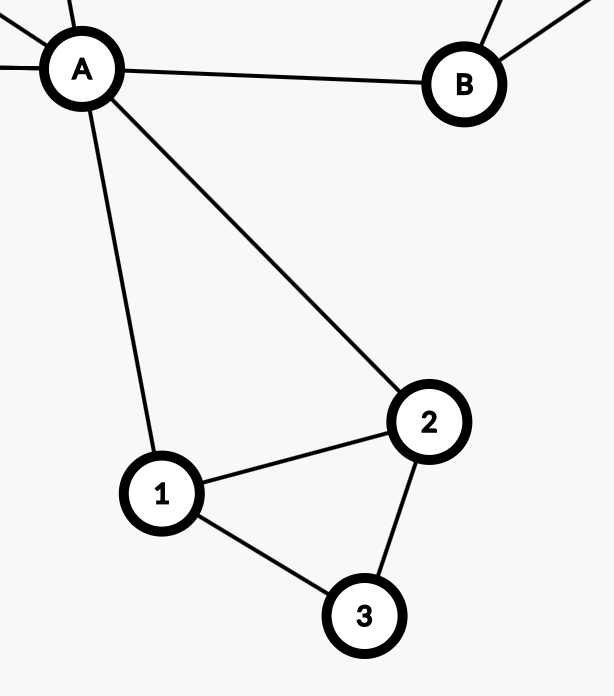
\includegraphics[width=\linewidth]{_img/340/01.png}
              \end{subfigure}
              \begin{subfigure}[a]{0.24\linewidth}
                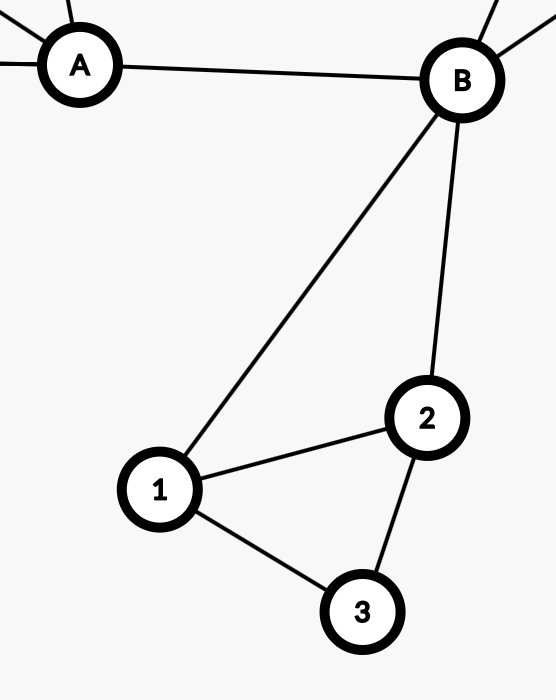
\includegraphics[width=\linewidth]{_img/340/02.png}
              \end{subfigure}
              \caption{Два возможных случая}
            \end{figure}
            Тут $\{1,2,3\}$ --- какой-то треугольник в графе $G$, а новый найденный треугольник в $G$ --- либо $\{A,1,2\}$, либо $\{B,1,2\}$.

            \item Пусть теперь из $A$ и $B$ идет в оставшуюся часть графа в совокупности меньше, чем $n - 2$ ребро. Имеем $|E'| \geq \left\lfloor\frac{{\left (n-2\right)}^2}{4}\right\rfloor - n + 2$. Удалим ребро одного из треугольников, не инцидентное $A$ или $B$. Теперь, в графе $|E| \geq \left\lfloor\frac{{\left (n-2\right)}^2}{4}\right\rfloor - n + 1$, значит, теперь в графе (по предположению индукции)~---~минимум $\left\lfloor\frac{n}{2}\right\rfloor - 1$ треугольник. Вернем ребро обратно и заметим, что оно образует недостающий треугольник, ведь удаленное ребро лежало в одном из треугольников до удаления.
        \end{enumerate}
    \end{enumerate}
\end{solution}

\begin{task}{344}
Перечислите все попарно неизоморфные связные простые графы на шести вершинах, в которых ровно три блока.
\end{task}

\begin{solution}
Разобьем графы на группы, для простоты и алгоритмичности перебора:
\begin{figure}[H]
  \centering
  \begin{subfigure}[a]{0.24\linewidth}
    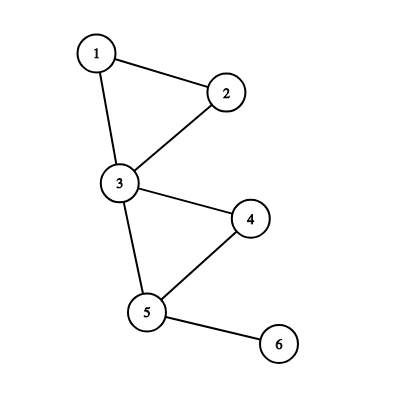
\includegraphics[width=\linewidth]{_img/344/01.png}
  \end{subfigure}
  \begin{subfigure}[a]{0.24\linewidth}
    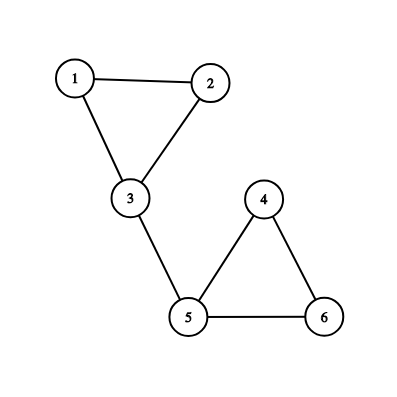
\includegraphics[width=\linewidth]{_img/344/02.png}
  \end{subfigure}
  \begin{subfigure}[a]{0.24\linewidth}
    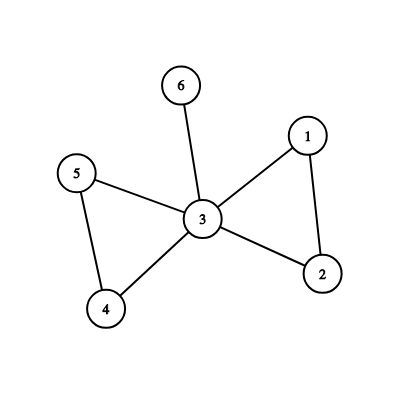
\includegraphics[width=\linewidth]{_img/344/03.png}
  \end{subfigure}
  \caption{Два треугольника и ребро.}
\end{figure}

\begin{figure}[H]
  \centering
  \begin{subfigure}[a]{0.24\linewidth}
    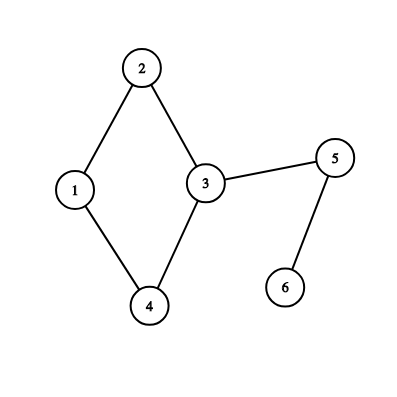
\includegraphics[width=\linewidth]{_img/344/04.png}
  \end{subfigure}
  \begin{subfigure}[a]{0.24\linewidth}
    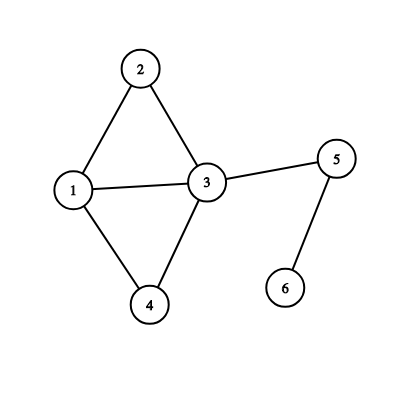
\includegraphics[width=\linewidth]{_img/344/05.png}
  \end{subfigure}
  \begin{subfigure}[a]{0.24\linewidth}
    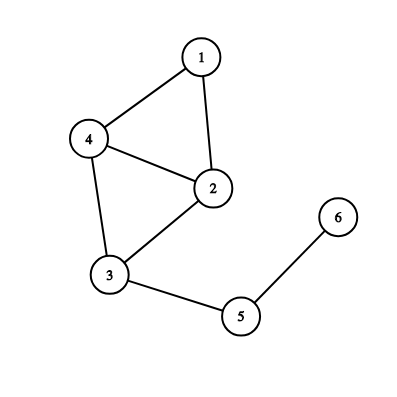
\includegraphics[width=\linewidth]{_img/344/06.png}
  \end{subfigure}
  \begin{subfigure}[a]{0.24\linewidth}
    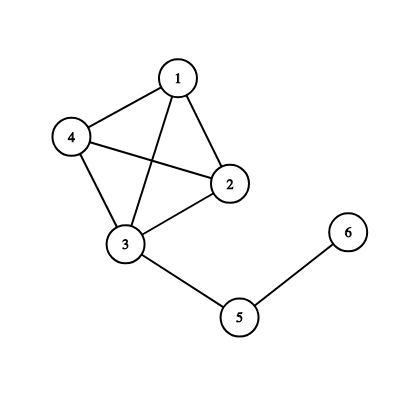
\includegraphics[width=\linewidth]{_img/344/07.png}
  \end{subfigure}
  \caption{Квадрат и два последовательных ребра.}
\end{figure}

\begin{figure}[H]
  \centering
  \begin{subfigure}[a]{0.24\linewidth}
    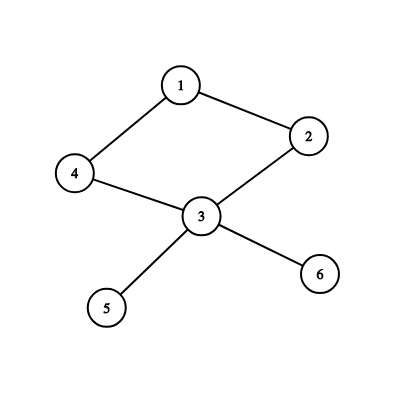
\includegraphics[width=\linewidth]{_img/344/08.png}
  \end{subfigure}
  \begin{subfigure}[a]{0.24\linewidth}
    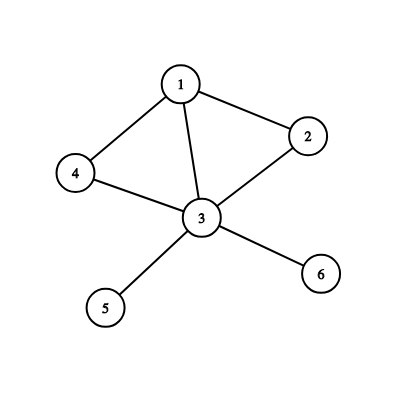
\includegraphics[width=\linewidth]{_img/344/09.png}
  \end{subfigure}
  \begin{subfigure}[a]{0.24\linewidth}
    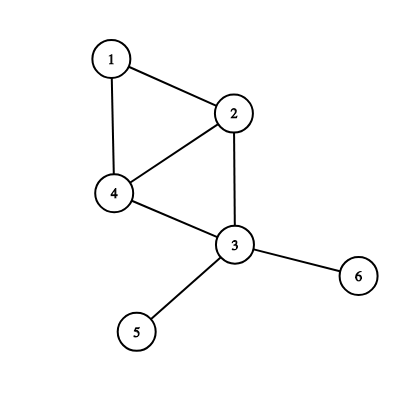
\includegraphics[width=\linewidth]{_img/344/10.png}
  \end{subfigure}
  \begin{subfigure}[a]{0.24\linewidth}
    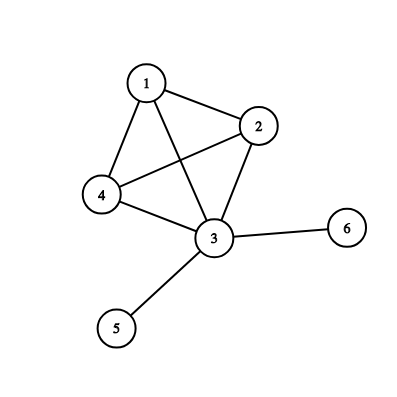
\includegraphics[width=\linewidth]{_img/344/11.png}
  \end{subfigure}
  \caption{Квадрат и два инцидентных ребра.}
\end{figure}

\begin{figure}[H]
  \centering
  \begin{subfigure}[a]{0.24\linewidth}
    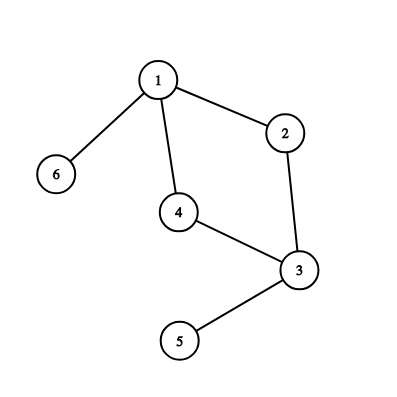
\includegraphics[width=\linewidth]{_img/344/12.png}
  \end{subfigure}
  \begin{subfigure}[a]{0.24\linewidth}
    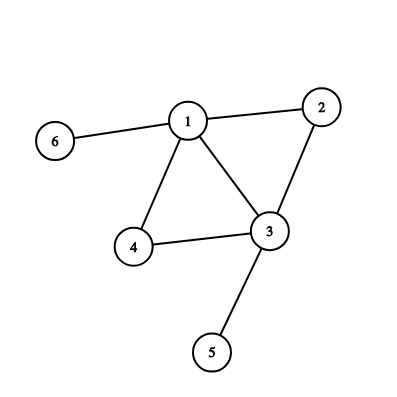
\includegraphics[width=\linewidth]{_img/344/13.png}
  \end{subfigure}
  \begin{subfigure}[a]{0.24\linewidth}
    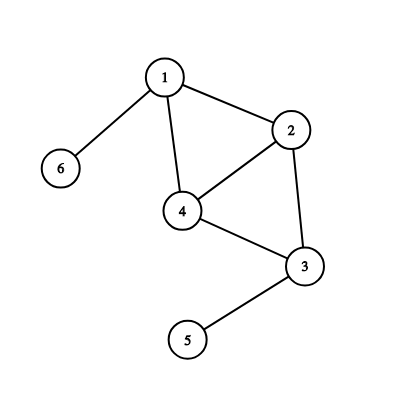
\includegraphics[width=\linewidth]{_img/344/14.png}
  \end{subfigure}
  \begin{subfigure}[a]{0.24\linewidth}
    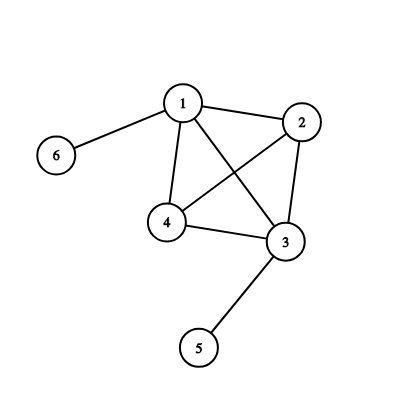
\includegraphics[width=\linewidth]{_img/344/15.png}
  \end{subfigure}
  \caption{Квадрат и два диаметрально противоположных ребра.}
\end{figure}

\begin{figure}[H]
  \centering
  \begin{subfigure}[a]{0.24\linewidth}
    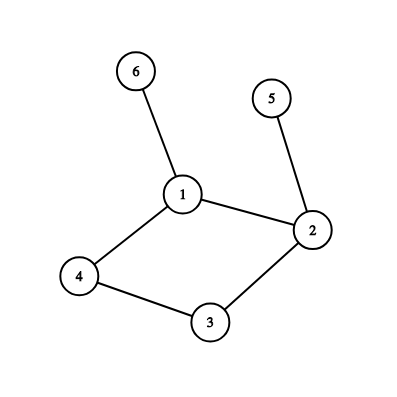
\includegraphics[width=\linewidth]{_img/344/16.png}
  \end{subfigure}
  \begin{subfigure}[a]{0.24\linewidth}
    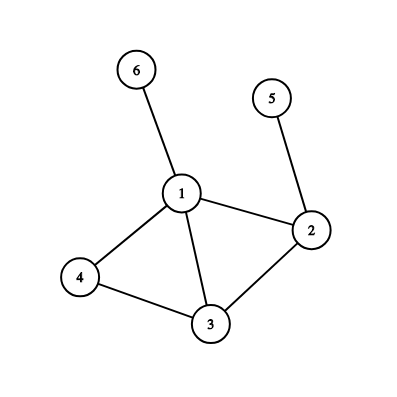
\includegraphics[width=\linewidth]{_img/344/17.png}
  \end{subfigure}
  \caption{Квадрат и два ребра.}
\end{figure}

Таким образом, искомых графов всего семнадцать.
\end{solution}

\end{document}
